\section{Resultados}

Se muestra a continuación los resultados numéricos obtenidos. En la Figuras \ref{fig_1} y \ref{fig_2} se muestra el campo de velocidad y de presión de la mitad inferior de la tubería. Se observan leves diferencia en los perfiles de velocidad: El primer caso presenta componentes verticales de velocidad mientras que en el segundo caso son prácticamente nulos. Notar que el gradiente de presión es aproximadamente el doble que en el segundo caso (lo que es relevante es la diferencia de presión, no la presión en sí)\\

En la Figura \ref{fig_3} se comparar los resultados de perfil de velocidad en $x=Lx/2$ para modificando la razón de proporción de los volúmenes. En la medida que se vuelven menos regulares (alejandose de la relación 1:1, $Lx=5$, $nx=50$, $Ly=1$, $ny=10$) los resultados se alejan de la solución analítica. \\

En la Tabla \ref{resultados_1} se determinan los número CFL que aseguran la estabilidad. Notar CFL disminuye en la medida que Re disminuye.

\begin{table}[H]
\centering
\begin{tabular}{|l|lll|} \hline
&Condición & 1 &  \\
Re & 2000	& 1500	& 1000 \\
CFL & 0.30	& 0.23	& 0.15 \\
T[s] & 18.908	& 45.036 & 19.840 \\ \hline
\end{tabular}
\begin{tabular}{|l|lll|} \hline
& Condición & 2 &  \\
Re & 2000	& 1500	& 1000 \\
CFL & 0.30	& 0.23	& 0.15 \\
T[s] & 124.16 & - & 90.427 \\ \hline
\end{tabular}
\caption{Número CFL que asegura la convergencia para cada Re ($Lx=5$, $Ly=1$, $Nx=50$, $Ny=10$). Condición 1: Presión impuesta en la entrada y salida; Condición 2: Condición periódica. El valor omitido es debido a que diverge para ese caso.} \label{resultados_1}
\end{table}


\begin{figure}[H]
\centering
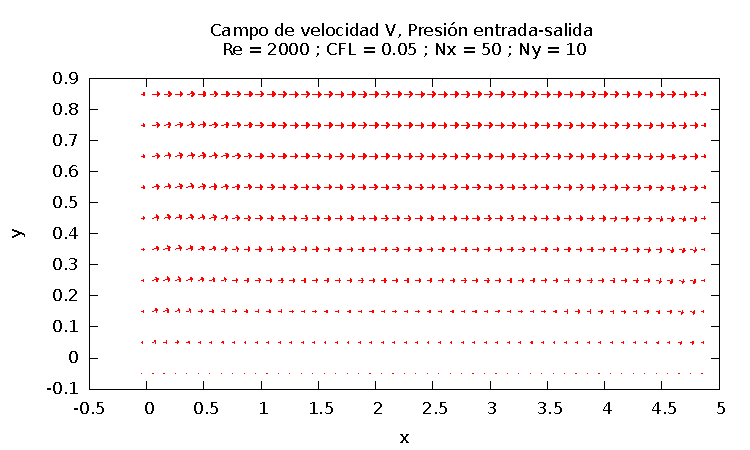
\includegraphics[width=1\textwidth]{./fig1_1/fig1_1/velocity_field.pdf}
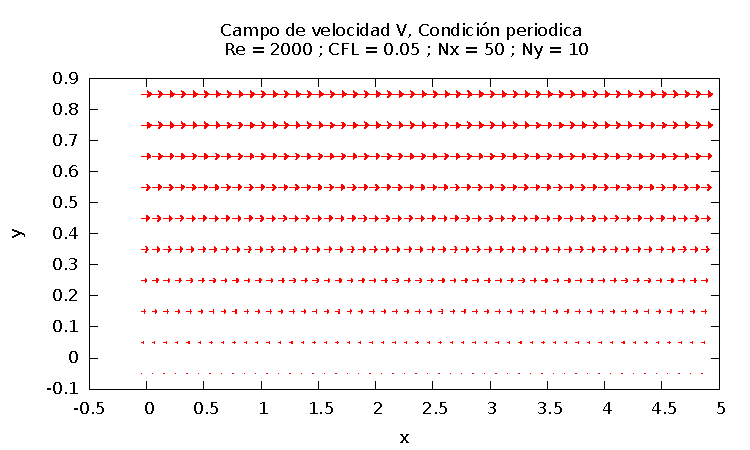
\includegraphics[width=1\textwidth]{./fig1_1/velocity_field.pdf}
\caption{Se observa que para el primer caso el perfil presenta componentes verticales del flujo} \label{fig_1}
\end{figure}

\begin{figure} [H]
\centering
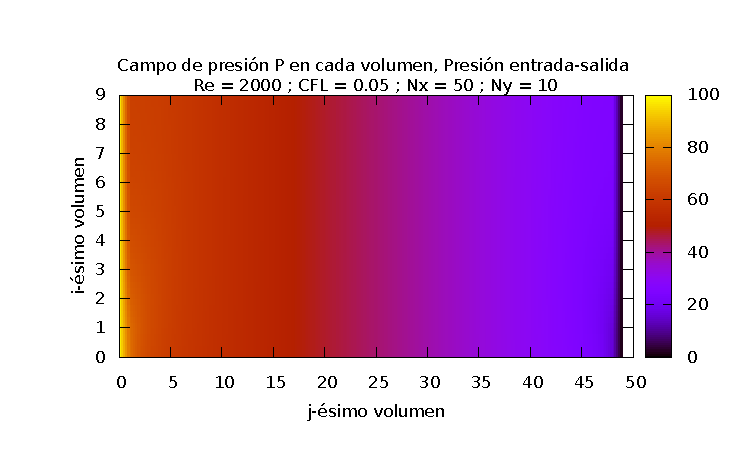
\includegraphics[width=1\textwidth]{./fig1_1/fig1_1/pressure_field.pdf}
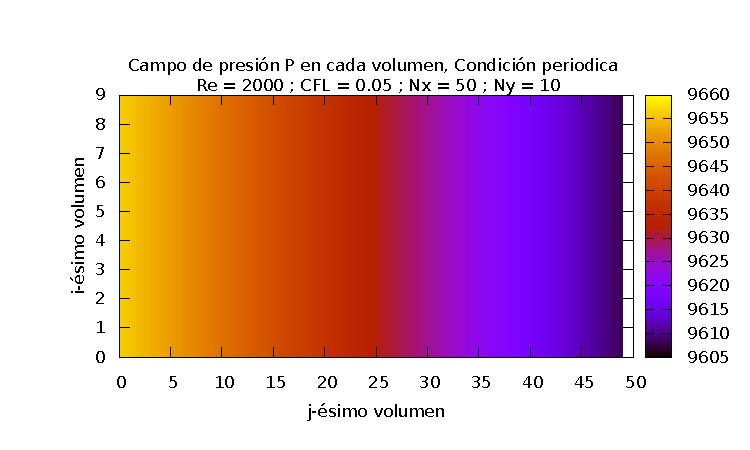
\includegraphics[width=1\textwidth]{./fig1_1/pressure_field.pdf}
\caption{El gradiente de presión en el primer caso es aproximadamente el doble que el segundo caso} \label{fig_2}
\end{figure}

\begin{figure} [H]
\centering
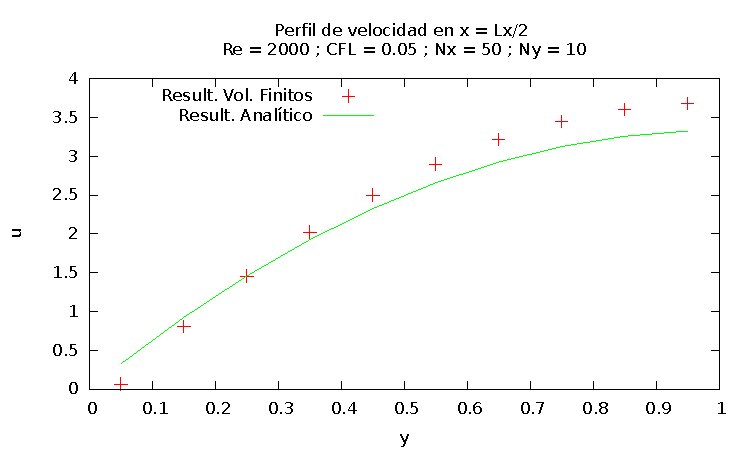
\includegraphics[width=0.8\textwidth]{./fig1_1/fig1_1/velocity_profile.pdf}
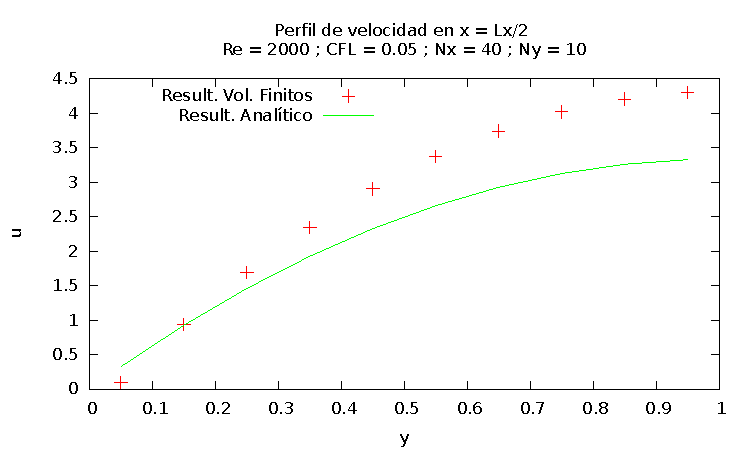
\includegraphics[width=0.8\textwidth]{./fig1_1/fig1_2/velocity_profile.pdf}
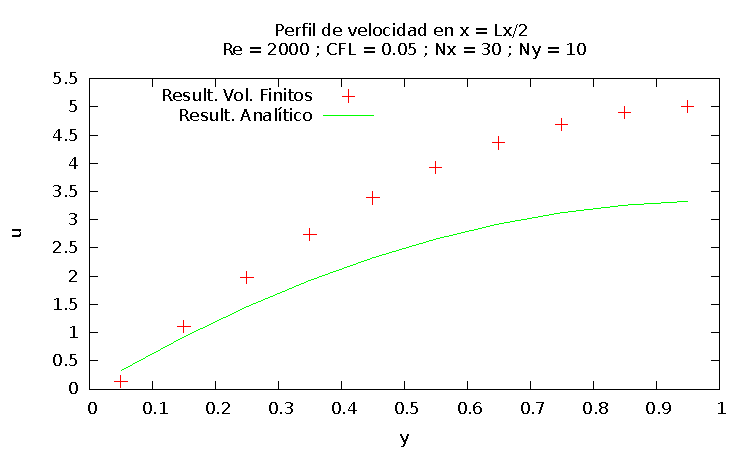
\includegraphics[width=0.8\textwidth]{./fig1_1/fig1_3/velocity_profile.pdf}
\caption{Perfil de velocidad en $x=L/2$ para distintos número de volumenes y distinta proporción geométrica.. } \label{fig_3}
\end{figure}
